%!TEX root = head.tex

\section{Empirical Results}
\label{sec:exp}

To demonstrate the practical value of our approach to checking observational
refinement, we argue that our symbolic refinement-checking algorithms
\begin{itemize}

  \item scale far beyond existing algorithms, and

  \item are often complete in practice.

\end{itemize}
To argue these points we have implemented several variations of three basic
refinement-checking algorithms for the membership query $h \in \overline{H}$.

\begin{description}

  \item[The Linearization Checker] enumerates the linearizations of $h$. For
  each (sequential) linearization $h' \succeq h$, we leverage an automated
  theorem prover to check whether $h'$ is included in the kernel $H$ via
  satisfaction query $h' |= \textsc{Theory}(H)$. If this check succeeds, we
  conclude that $h \in \overline{H}$. If this check fails for all of the
  linearizations $h'$ of $h$, we conclude that $h \not\in \overline{H}$.

  \item[The Satisfiability Checker] essentially delegates the enumeration of
  linearizations to an underlying theorem prover by encoding the refinement
  query into a logical question including the formula $\textsc{Theory}(H)$. As
  described in Section~\ref{sec:propositional}, we check $h \in \overline{H}$
  by checking the satisfiability of the formula $\textsc{Stronger}(h) /|
  \textsc{Theory}(H)$. If this check succeeds or is inconclusive, we conclude
  that $h \in \overline{H}$. If unsatisfiability is found, we conclude that $h
  \not\in \overline{H}$.

  \item[The Saturation Checker] avoids the expensive propositional
  branching/backtracking inherent to the aforementioned satisfiability query,
  by limiting the satisfiability check to Boolean constraint propagation.
  Essentially, we implement a solver which only saturates with unit
  propagation, avoiding any propositional branching. If a contradiction is
  found, we conclude that $h \not\in \overline{H}$. Otherwise if saturation
  fails to reveal a contradiction, we conclude $h \in \overline{H}$.

\end{description}

We have studied actual concurrent data structure implementations, including the
Scal\footnote{\url{http://scal.cs.uni-salzburg.at}} High-Performance
Multicore-Scalable Computing suite. Some of these implementations, such as the
Michael-Scott Queue~\cite{conf/podc/MichaelS96}, are meant to preserve
observational refinement\footnote{More precisely, they are designed to be
linearizable.}, while others, such as the non-blocking bounded-reordering
queue~\cite{conf/pact/KirschLP13}, are meant to preserve weaker properties.

The input to our checking algorithms are histories given as text files
consisting of line-separated call and return actions. For the selected set of
concurrent object implementations, we generated the histories of several
pseudo-random executions by logging calls and returns in the order in which
they occurred. While scanning an input history, the selected algorithm performs
a membership test at each prefix at which an operation completes --- i.e.,~at
return actions.

Our first set of experiments (\S\ref{sec:exp:scalable}) demonstrates that our
symbolic algorithms are drastically more scalable than existing algorithms, in
that they are able to process vastly more history operations in much shorter
time. Our second set of experiments (\S\ref{sec:exp:complete}) demonstrates
that while our more efficient algorithms can be incomplete on certain
hand-crafted cases, failing to identify particularly intricate refinement
violations, the violations surfacing in the logs of actual executions are
consistently discovered. We made all measurements on similar MacBook Proc
2.XGHz Intel Core i5/i7 machines, and discharged theorem-prover queries with
Z3 version 4.3.1.

\subsection{Scalability of Symbolic Checking}
\label{sec:exp:scalable}

TODO ARGUE THAT WE'RE EXTREMELY SCALABLE

\subsection{Completeness in Practice}
\label{sec:exp:complete}

TODO ARGUE THAT WE AREN'T MISSING VIOLATIONS


\begin{table}[t]
  \footnotesize
  \centering
  \setlength{\tabcolsep}{1.8mm}
  \begin{tabular}{ccccc}
   & Nb. of steps  & & Nb. of & Step of  \\
   Method & to timeout & Time & violations & the violation \\
  \hline
  Lineup & 35 & - & 0/4 \\
  Lineup -c & 38 & - & 0/4 \\
  SMT & 52 & - & 3/4 & 39, 49, 51\\
  SMT -r & 52 & - & 3/4 & 39, 49, 51\\
  SMT -i & 51 & - & 3/4 & 39, 49, 51\\
  SMT -c & 38 & - & 0/4 \\
  SMT -c -i & 38 & - & 0/4 \\
  Saturation & 100 & 0.1340s & 4/4 & 39, 49, 51,100\\
  Saturation -r  & 100 & 0.1521s & 4/4 &39, 49, 51,100 
  %MSQueue                             & 2xEnqueue 2xDequeue & 0 & 2 & 2 & & Yes \\
  \end{tabular} 
  \caption{Experimental data for the very concurrent {\tt bkq} and {\tt msq}: 200 executions and only 4 violations.
  Timeout is set to 5 seconds.
    }
  \label{tab:exp:concur}
\end{table}


\begin{table}[t]
  \footnotesize
  \centering
  \setlength{\tabcolsep}{1.8mm}
  \begin{tabular}{cccc}
   	        & 	                     & Step of     \\
   Method & $\%$ violations  & violations & Time \\
  \hline
  Lineup & 55$\%$ & 23.8 & 1.2593s \\
  Lineup -c & 88$\%$ & 23.8 & 0.8906s \\
  SMT & 75$\%$ & 23.8 & 1.1058s \\
  SMT -r & 78$\%$ & 23.8 & 0.8390s\\
  SMT -i & 90$\%$ & 23.8 & 0.5053s\\
  SMT -c & 100$\%$ & 23.8 & 0.8461s \\
  SMT -c -i & 100$\%$ & 23.8 & 0.5021s \\
  Saturation & 100$\%$ & 24.2 & 0.0171s\\
  Saturation -r  & 100$\%$ & 24.2 & 0.0191s
  %MSQueue                             & 2xEnqueue 2xDequeue & 0 & 2 & 2 & & Yes \\
  \end{tabular} 
  \caption{Experimental data for the very sequential {\tt bkq}: 100 executions which are all violations. The column ``Step of violations'', resp., ``Time'',
  gives the step at which a method found the violation and the time spent, in average, but only for the 53 violations
  which were detected by all methods. In 9 cases, the saturation procedure is late to detect a violation by two steps
  from 21 to 23. Timeout is set to 5 seconds.
    }
  \label{tab:exp:sec}
\end{table}


\begin{figure}[t]
  \centering
  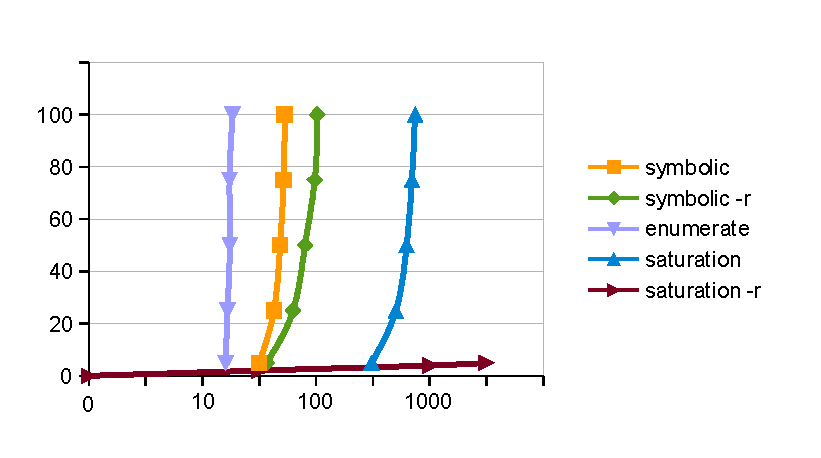
\includegraphics[width=\linewidth]{figures/new_chart}
  \caption{Logarithmic scale. Lineup -r behaves like lineup. The other smt -i, smt -i -c, smt -c behave like smt.
  }
  \label{fig:data:chart}
\end{figure}






